\subsection{}

\begin{definition}
    \emph{Law of demand} says \underline{ceter}is \underline{par}ibus, meaning all things equal. Demand is consumer-driven.
    As the price of something goes up, your willingness to buy it goes down. The reverse is true too,
    as the price of something goes down, your willingness to buy it goes up.\\
    Note: Technically, the law of demand is as the price of something goes up, your willingness to buy it \emph{should not} increase.
\end{definition}
\begin{definition}
    Demand Schedule is a table that shows prices and quantities. Graphing the demand schedule has the 
    quantity as the dependent variable and the price as the independent variable. Even though this is the case,
    Price is on the dependent axis (y-axis) and quantity on the independent axis (x-axis).
\end{definition}
\begin{figure}[H]
    \centering
    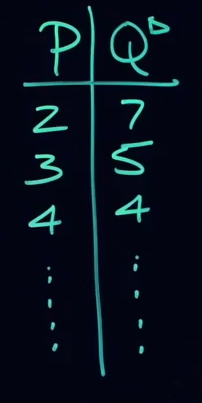
\includegraphics[]{Chapter3/DemandScheduleTable.png}
    \caption{Demand Schedule}
\end{figure}
\begin{definition}
    Demand curve is a graphical representation of the demand schedule. Price is on the y-axis and quantity on the x-axis.
    It is a downward sloping curve, but in the real world it is not always. It is drawn linearly for simplicity, this comes with a problem.
    If the price was free (y=0) it would break the law of demand. Assume the demand curve is for the entire market for the product.
\end{definition}
\begin{figure}[H]
    \centering
    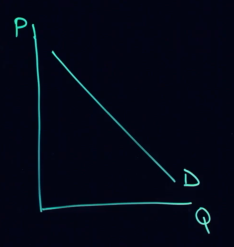
\includegraphics[]{Chapter3/DemandCurve.png}
    \caption{Demand Curve}
\end{figure}
\begin{definition}
    A \emph{shift} in demand is when other factors besides price change.
\end{definition}
\begin{example}
    If your incomes goes up, given the same price of a product, you would want to purchase more of it. (normal good)\\
    Note: There are some goods that you would want to purchase less of if your income goes up (inferior goods). In this event, there would be a left shift.\\
    The demand curve would shift to the right.\\ If a substitute product's price goes up, 
    you would want to purchase more of the original product.
    \begin{figure}[H]
        \centering
        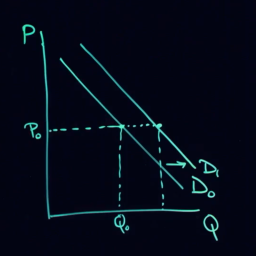
\includegraphics[]{Chapter3/DemandCurveShift.png}
        \caption{Demand Curve Shifts to Right}
    \end{figure}
    If the price of a complementary product goes up, you would want to purchase less of the original product (left shift).\\
    If the price expectation (future price) goes up, you would want to purchase more of the product now.\\
    If the number of consumers increases, demand curve shifts right.\\
    All the above scenarios cause a change in demand.\\
    If the price of the product goes up, the demand curve does not shift. This is only a change in quantity demanded.
\end{example}
\begin{figure}[H]
    \centering
    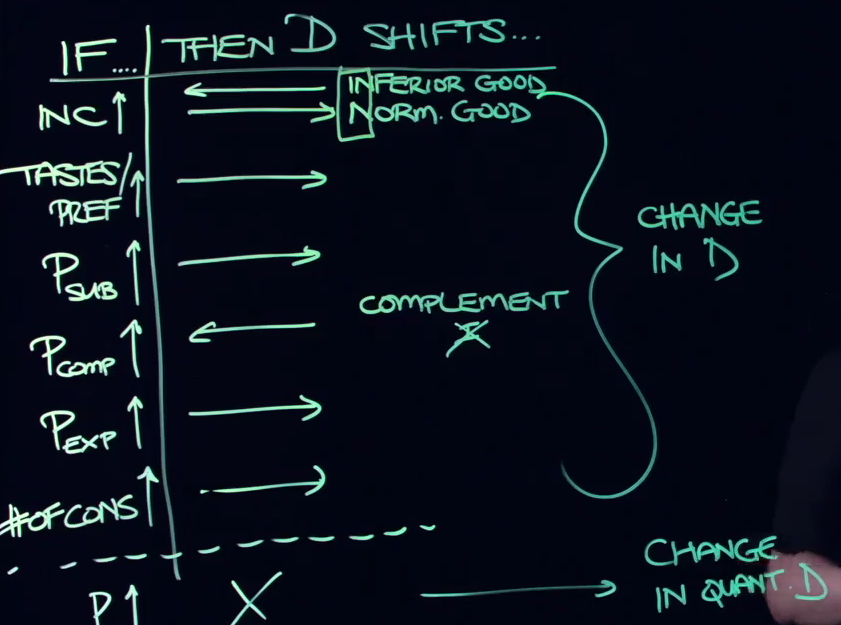
\includegraphics[]{Chapter3/ShiftExamples.png}
    \caption{Demand Shift Examples}
\end{figure}